% --- chapter4.tex ---
\chapter{Design}
\label{chap:design}

This chapter presents the system analysis and design of our VR-based mental health therapy platform. It describes the architecture, workflow, data structure, software classes, and the graphical user interface. Our design emphasizes scalability and usability, also integrating AI components for session handling.

\section{System Architecture}
Our system follows a client-server architecture. The frontend captures user input and displays simulations. It communicates with the backend through APIs. The backend consists of three layers: the application layer for managing session workflows, the AI service layer for conversation and tagging tasks, and the data layer storing all session and analysis information in MongoDB. This separation ensures maintainability and secure communication.

\begin{figure}[H]
\centering
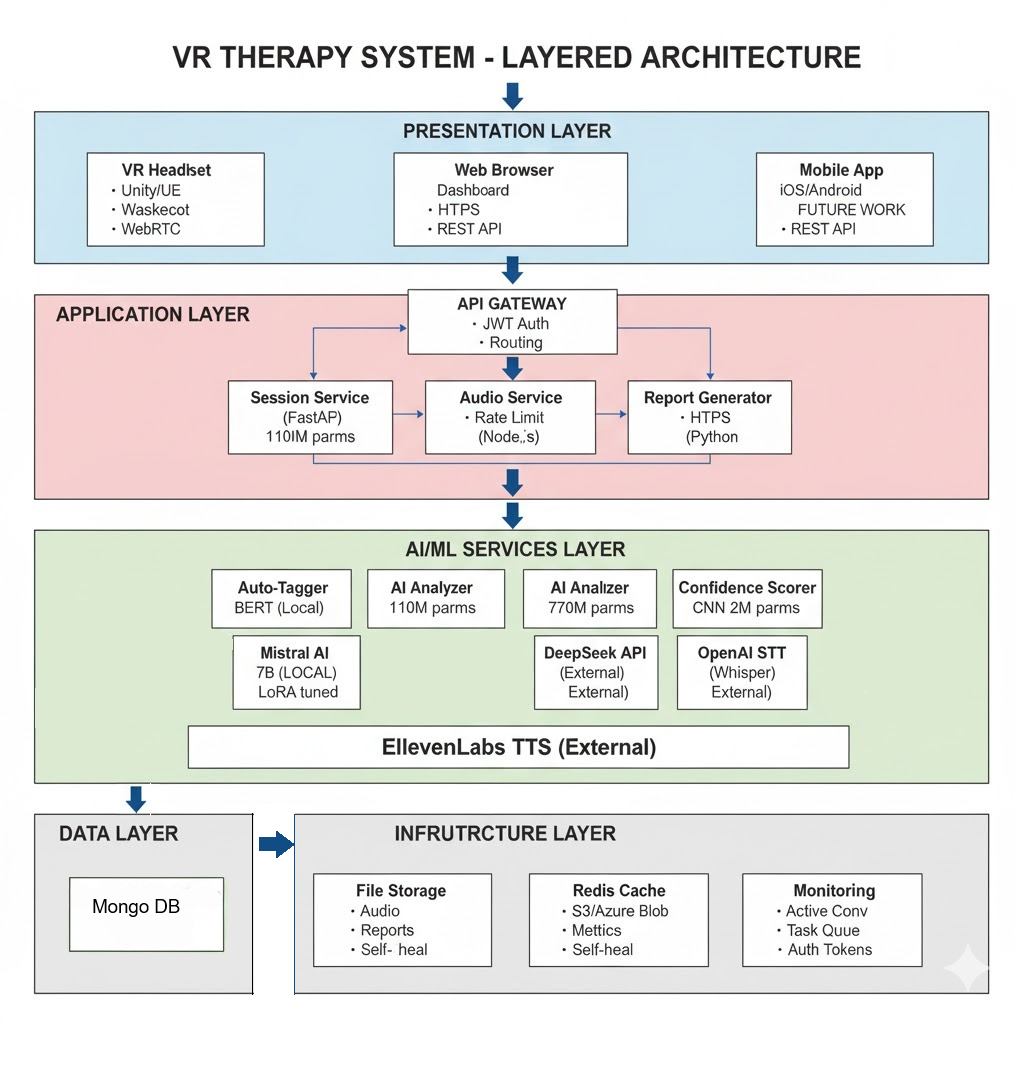
\includegraphics[width=0.9\textwidth]{figures/Layered artitecture.png}
\caption{Layered architecture of VR Therapy System.}
\label{fig:system_architecture}
\end{figure}

\section{Activity Diagram}
The activity diagram (Figure \ref{fig:activity_diagram}) represents the sequential workflow of a complete session. The process begins when a user starts a new session, providing information on issue, intensity, and voice input. The system then enters the AI conversation loop, which performs auto-tagging and condition analysis. It selects an appropriate VR simulation, delivers the simulation, captures post-session feedback and scores, and saves the report in the database.

\begin{figure}[H]
\centering
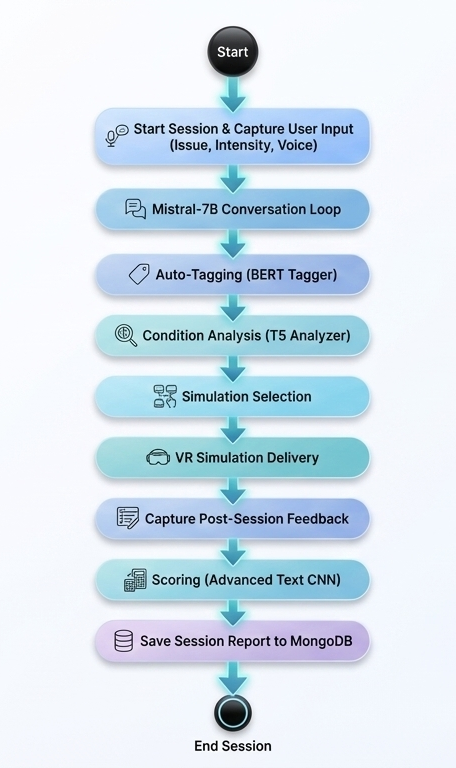
\includegraphics[width=0.5\textwidth]{figures/Activity Diagram.png}
\caption{Activity diagram of the therapy session workflow.}
\label{fig:activity_diagram}
\end{figure}

\section{ER Diagram}
The Entity Relationship (ER) diagram (Figure \ref{fig:er_diagram}) represents the database schema. The \textbf{User} entity serves as the central point for all data relations. It includes attributes such as Name, Email, Age, and Department/Role and represents the individual seeking mental health support. Each User can generate multiple chat logs stored in the \textbf{Chat\_Log} entity, which records timestamp, message content, and sender info. The \textbf{AI\_Model} entity represents the AI engines processing the chat logs, with attributes including Model Type, Version, and Accuracy Score. Analytical outputs such as Risk Level, Summary Content, and generation dates are stored in the \textbf{Report} entity. Users can schedule appointments via the \textbf{Counselling\_Session} entity, conducted by a Counsellor with Name, Specialization, and Contact Info. Users provide feedback recorded in the \textbf{Feedback} entity, which includes Rating, Comments, and Submission Date.

\begin{figure}[H]
\centering
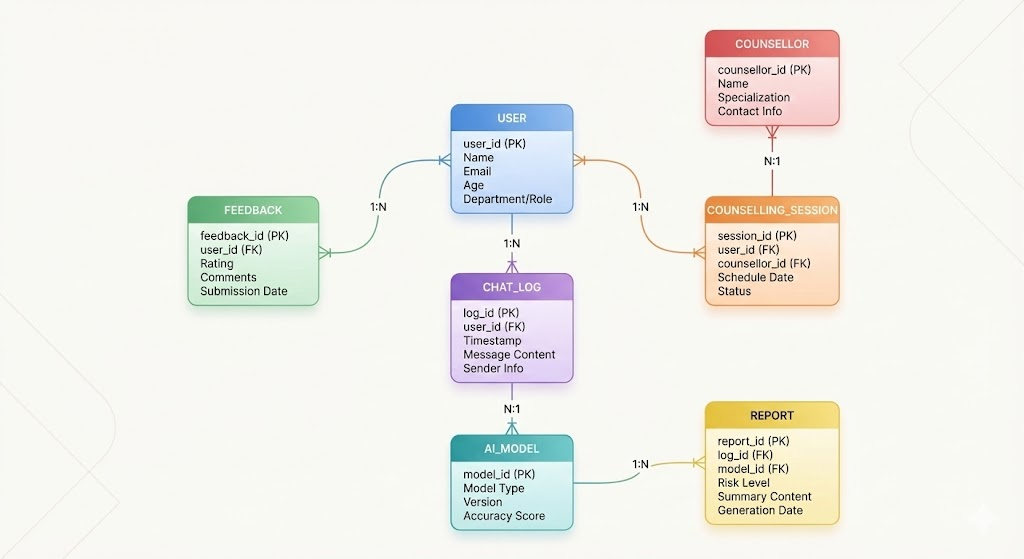
\includegraphics[width=0.8\textwidth]{figures/ER DIAGRAM.png}
\caption{Entity Relationship Diagram of the VR therapy system.}
\label{fig:er_diagram}
\end{figure}

\section{Class Diagram}
The Class Diagram (Figure~\ref{fig:class_diagram}) represents the software objects used within our project. It follows Object-Oriented Programming (OOP) principles and shows major classes, their attributes, methods, and relationships that define the system’s behavioral and structural architecture. The diagram is divided into user-level classes, system logic and analysis classes, therapy and VR simulation classes, and utility/backend management classes.

\paragraph{User-Level Actor Classes}
At the core of the actor hierarchy is the \textbf{User} class, defining fundamental properties and functionalities shared by all individuals interacting with the system. Attributes include \textit{UserID}, \textit{Name}, \textit{Email}, and \textit{Password}, with methods \textit{Login()}, \textit{Logout()}, and \textit{UpdateProfile()}.  

Two classes extend the base class:
\begin{itemize}
    \item \textbf{Student} (or Client) represents individuals seeking counseling services. Attributes: \textit{StudentID}, \textit{Department}, \textit{Age}. Methods: \textit{StartChat()}, \textit{BookSession()}, \textit{ViewReport()}.
    \item \textbf{Counsellor} models practitioners guiding therapy sessions. Attributes: \textit{CounsellorID}, \textit{Specialization}, \textit{AvailableSlots}. Methods: \textit{ViewStudentData()}, \textit{ApproveSession()}, \textit{WriteSessionNotes()}.
\end{itemize}

\paragraph{Communication and Interaction Classes}
\begin{itemize}
    \item \textbf{ChatSystem} handles real-time text communication, storing chat data via \textit{ChatID}, \textit{Timestamp}, and \textit{MessageLog}, and processes messages, displays responses, and archives history.
    \item \textbf{VRInteractionManager} handles in-environment interactions and navigation within VR therapy spaces.
    \item \textbf{VoiceProcessor} orchestrates voice-related tasks and delegates responsibilities to \textbf{SpeechToText} (audio to text) and \textbf{TextPreprocessor} (cleans and structures text for ML analysis).
\end{itemize}

\paragraph{AI and Analysis Layer}
\begin{itemize}
    \item \textbf{AI\_Analyzer} interprets user messages; attributes: \textit{ModelVersion}, \textit{ConfidenceThreshold}; methods: preprocess text, analyze sentiment, detect risk factors, generate AI responses.
    \item \textbf{AutoTagger} assigns semantic, emotional, or psychological tags; supported by \textbf{TagModel} storing model weights and configurations.
    \item \textbf{ConditionAnalyzer} evaluates conversation context, infers emotional states, and aids in thematic summaries.
\end{itemize}

\paragraph{Therapy Selection and VR Simulation Classes}
\begin{itemize}
    \item \textbf{TherapySelector} maps emotional/behavioral assessments to suitable VR interventions.
    \item \textbf{TherapyModule} defines environment types, therapeutic goals, and parameters.
    \item \textbf{SimulationManager} controls session timing and in-VR stimuli presentation.
\end{itemize}

\paragraph{Evaluation and Reporting}
\begin{itemize}
    \item \textbf{EvaluationManager} assesses feedback, emotional responses, and behavioral changes.
    \item \textbf{ReportGenerator} compiles conversation history, analysis results, therapy decisions, and evaluations into structured formats.
\end{itemize}

\paragraph{Utility, Data Management, and System Support}
\begin{itemize}
    \item \textbf{SessionManager} oversees scheduling and administration of VR and text-based therapy sessions.
    \item \textbf{DatabaseManager} handles data persistence and CRUD operations.
    \item \textbf{Logger} captures system events, errors, and activity logs.
\end{itemize}

\paragraph{Relationships and Multiplicities}
A single User may initiate multiple chat sessions through the ChatSystem, each processed by an AI\_Analyzer instance. Outputs from AI\_Analyzer, AutoTagger, and ConditionAnalyzer feed into TherapySelector and ReportGenerator. Students and Counsellors interact with SessionManager for bookings and approvals. VR simulation components engage with analysis outputs and user interactions. All components depend on DatabaseManager, and Logger records activities across modules.

\begin{figure}[H]
\centering
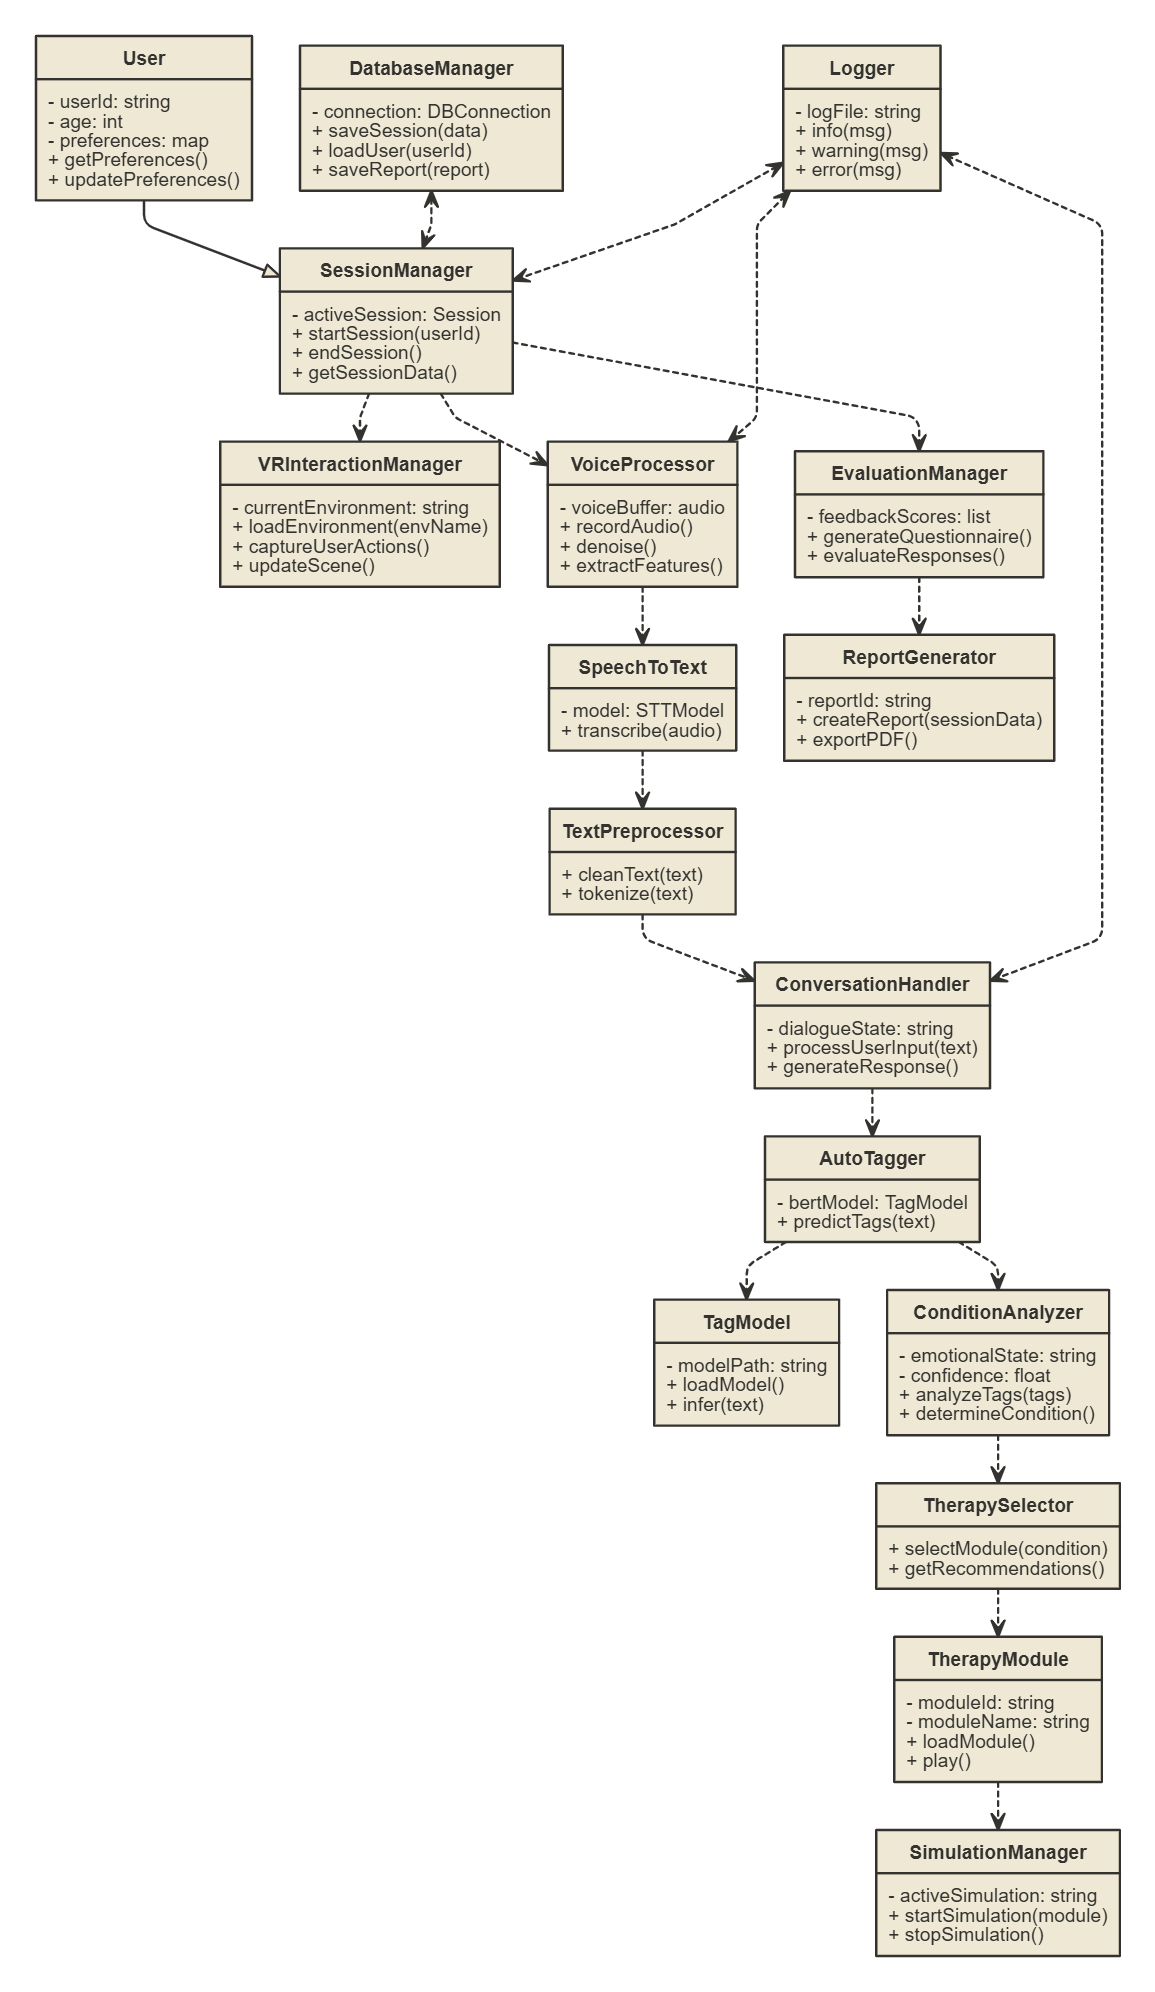
\includegraphics[width=0.7\textwidth]{figures/Class Diagram.png}
\caption{Class Diagram of the VR therapy system.}
\label{fig:class_diagram}
\end{figure}

\section{GUI Design}
The VR frontend is designed for professional and user-friendly interactions. Users input issue type and intensity; the system recommends simulations such as Relaxation, Exposure Therapy, Cognitive Behavioral Therapy, Mindfulness, and Social Interaction Simulation. Intensity is classified as mild, moderate, hard, or extreme. Post-session feedback is captured for evaluation. Interface provides a simple panel for speaking, receiving AI responses, viewing recommended simulations, and ending sessions.

\begin{figure}[H]
\centering

\includegraphics[width=0.9\textwidth]{dashboard.jpg}
\caption{System Login and Landing Page}
\label{fig:dashboard}
\end{figure}

\begin{figure}[H]
\centering

\includegraphics[width=0.9\textwidth]{Admin.jpg}
\caption{Admin Dashboard Overview and Analytics}
\label{fig:admin_panel}
\end{figure}

\begin{figure}[H]
\centering

\includegraphics[width=0.9\textwidth]{User Managment.jpg}
\caption{User Management Interface for Administrators}
\label{fig:user_mgmt}
\end{figure}

\begin{figure}[H]
\centering

\includegraphics[width=0.9\textwidth]{User Side.jpg}
\caption{User Chat Interface for Therapy Sessions}
\label{fig:user_side}
\end{figure}

\begin{figure}[H]
\centering

\includegraphics[width=0.8\textwidth]{VR 1ST Scene.jpg}
\caption{VR Application Initialization and Welcome Screen}
\label{fig:vr_scene_1}
\end{figure}

\begin{figure}[H]
\centering

\includegraphics[width=0.9\textwidth]{VR 2ND AND 4TH SCENE.jpg}
\caption{VR Therapy Room Environment and Simulation}
\label{fig:vr_scene_2_4}
\end{figure}

\section{Summary}
This chapter presented the system analysis and design of the VR-based mental health therapy platform. It described the architecture, workflow, ERD, class diagram, and GUI design. The activity diagram illustrates the therapy session flow, the ERD details all entities and their relationships with the User as the central point, and the class diagram shows core actor classes, system logic classes, and their interactions. Together, these models provide a detailed blueprint for implementing the system in the next chapter.
